\documentclass[a4paper]{article}


\usepackage[T2A]{fontenc}
\usepackage[utf8]{inputenc}
\usepackage[english,russian]{babel}

\usepackage{graphicx}
\graphicspath{{pictures/}}
\DeclareGraphicsExtensions{.pdf,.png,.jpg}

\usepackage{amsmath, amsfonts, amssymb, amsthm, mathtools}

\author{Шорин Сергей, БКНАД211}
\title{Дискретная математика дз 5}
\date{\today}

\begin{document}

\maketitle

\newpage

\section*{1}
В дереве на 10 вершинах ровно три вершины имеют степень один. Сколько
вершин имеют степень три?

Рассмотрим дерево на 9 вершин, в котором ровно 2 вершины имеют степень один. В нем только два листа, следовательно, остальные 8 вершин будут располагаться на между ними (на пути между ними). Такой граф можно нарисовать в виде линии.

 Добавим вершину степени 1. Ее можно добавить либо к крайним вершинам (тогда будет всего 2 вершины степени 1, условие не выполняется), или добавить к любой вершине степени 2 - тогда в графе будет 3 вершины степени 1 и 1 вершина степени 3.
 
(Альтернативное решение - составить уравнение. Дерево имеет 9 ребер - следовательно, сумма степеней вершин равна  18. Так как всего 3 вершины степени 1, не может быть вершин со степенью больше 3.
Составим уравнение: $18 = 3 * 1 + n * 3 + (10 - 3 -n) * 2$, где n - количество вершин степени 3. $n = 1$)
\subsection*{Ответ}
В графе одна такая вершина.
 

\section*{2}
Найдите наибольшее количество вершин в связном графе, сумма степеней
вершин в котором равна 20.

В связанном графе на n вершинах должно быть не менее n - 1 ребро.


Так как в заданном графе сумма степеней вершин равна 20, в этом графе 10 ребер.

Из 10 ребер можно построить максимум связанный граф на 11 вершинах (линия) - при добавлении любой новой вершины граф перестает быть связанным.

\subsection*{Ответ}
В графе может быть максимум 11 вершин.

\section*{3}
В связном графе на n вершинах нет мостов. Какое наименьшее число рёбер
может быть в таком графе?

Допустим, в графе n ребер. Тогда можно построить циклический связанный граф, в котором все вершины будут иметь степень 2 - в таком графе нет мостов.

Уберем одну вершину и посчитаем, какие степени могут быть у вершин.

Сумма степеней графа - 2n. Всего n - 1 вершин. Следовательно, хоть одна(хоть две) вершина должна иметь степень 1 - то есть соединяться с основной частью графа мостом.

Следовательно, в графе с n-1 ребром обязательно будут мосты.

\subsection*{Ответ}
Минимум n ребер

\section*{4}
Существует ли связный граф, что степени всех его вершин чётные и в графе
есть мост?


Если в графе есть мост, то при его удалении в графе появится минимум 2 компоненты связанности. В каждой такой компоненте сумма степеней вершин будет равна 2n, где n- количество ребер в компоненте.

Вернем мост на место. В таком случае сумма степеней вершин в этой компоненте связанности станет равна 2n + 1, что очевидно не четно - следовательно, в этом графе есть вершины с нечетной степенью.

\subsection*{Ответ}
Такой граф не существует.

\section*{5}

Докажите, что если в графе есть не менее 6 вершин, то либо он сам, либо его
дополнение содержит цикл длины три.

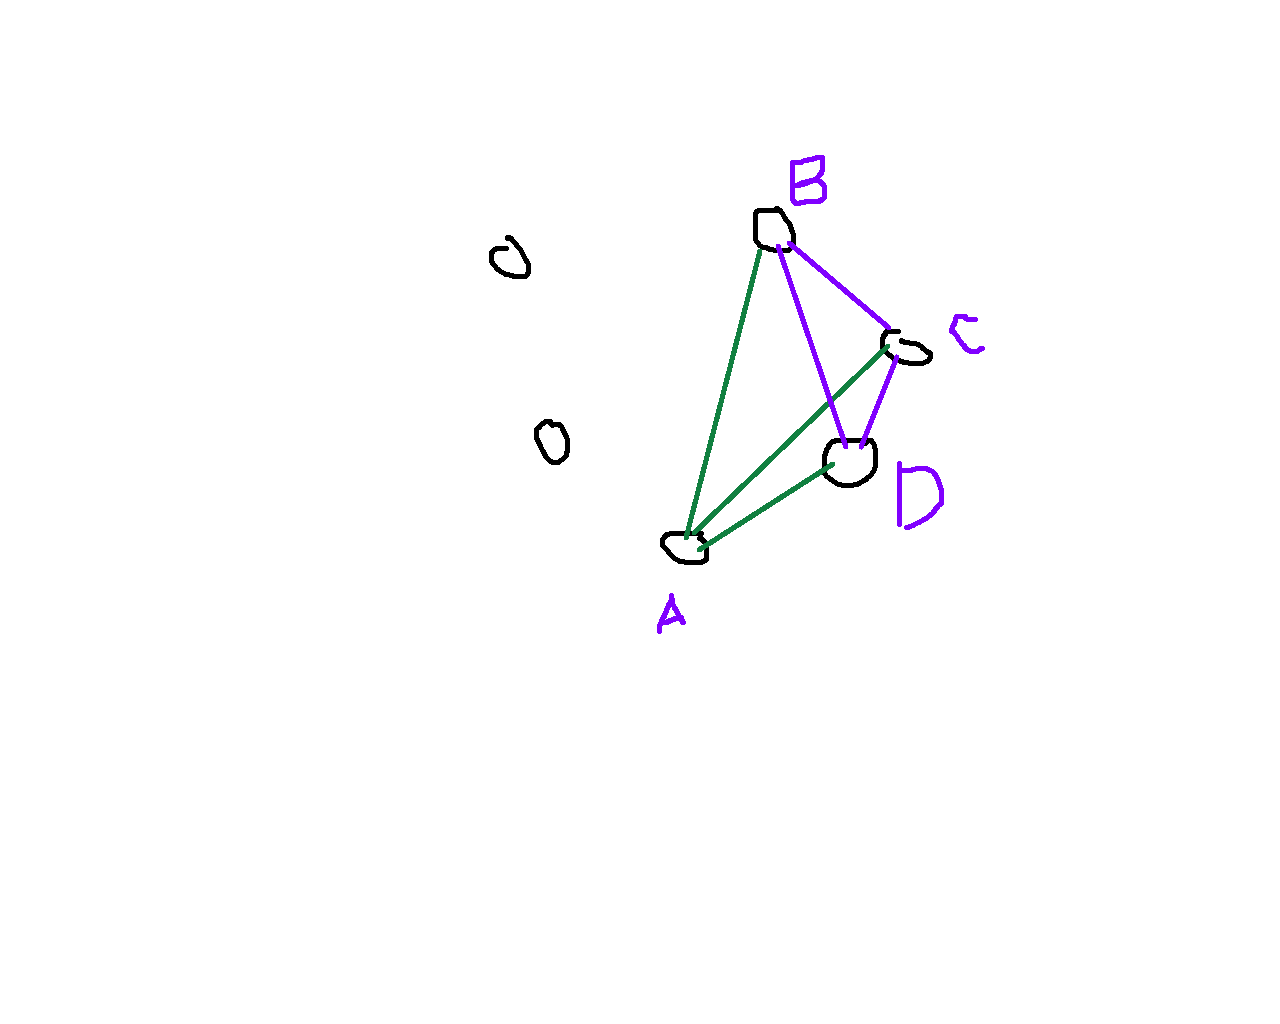
\includegraphics[width=12cm]{1}



Рассмотрим вершину А. Кроме нее в графе 5 вершин - значит, либо в этом графе, либо в его дополнении эта вершина соединена с 3 другими вершинами (или большем количеством).
Если вершина А соединена с другими вершинами в дополнении графа - дальше будем рассматривать дополнение как оригинальный граф.

Пусть это вершины B, C, D. Допустим, между ними нет ребер. Тогда в графе -дополнении они образуют цикл длиной 3 (BCD). Иначе в текущем графе есть хоть одно ребро между вершинами BCD. Допустим, это ребро MN ( $M, N \in [B, C, D]$). Тогда в графе образуется цикл длинной 3 (AMN).
В любом случае в графе образуется цикл длины 3, что и требовалось доказать.







\end{document}